\documentclass{article}
\usepackage[utf8]{inputenc}
\usepackage[margin=1in]{geometry}
\usepackage{graphicx}

\title{Math Clinic Status Update 4}
\author{Team 1: Komi Agbo, Dalton Burke, Nick Mako, James Vance}
\date{November 20th, 2019}

\begin{document}

\maketitle

\section{Since our last update...}
We have added visualizations to the route assignment algorithm, and made some
optimizations. The routes look valid for the most part, though there are some
strange things, such as some nodes appearing to have degree 3.

\begin{center}
	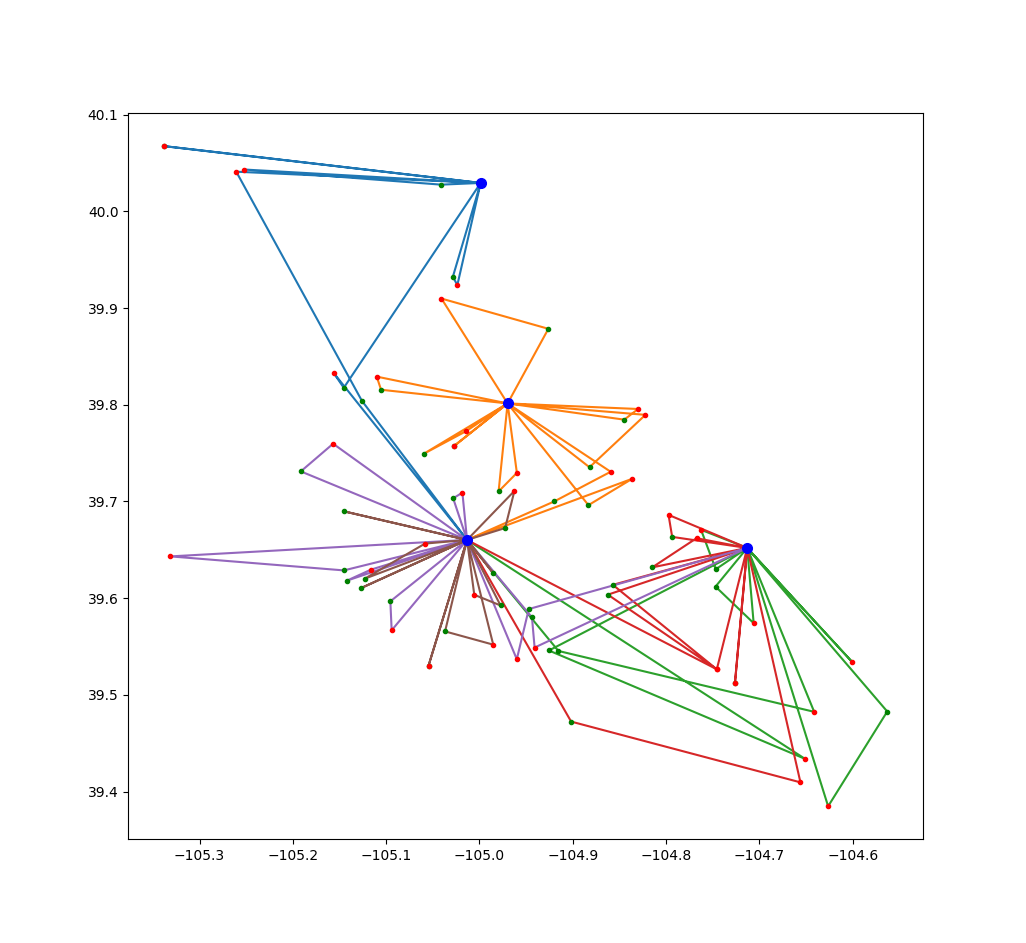
\includegraphics[scale=.55]{img/unrestricted_300.png}\\
	Route visualization, each worker doing only 300 minutes of driving, 
	each color represents a drivers route. No delivery-pickup zone
	restriction.\\
	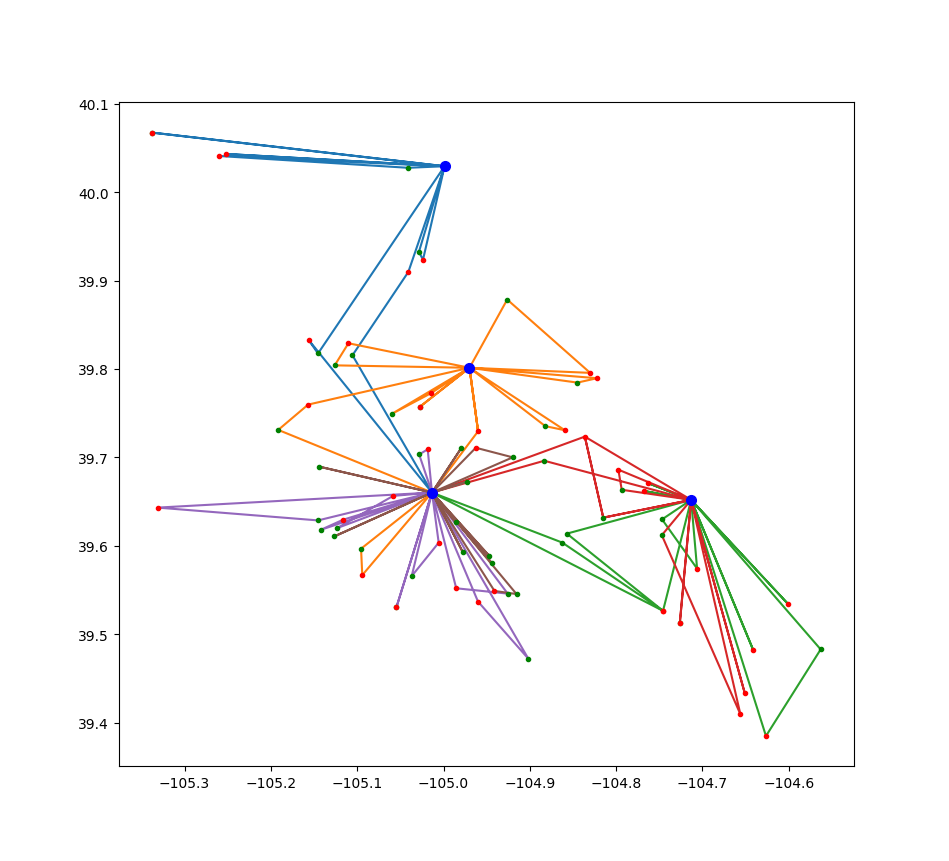
\includegraphics[scale=.55]{img/restricted_300.png}\\
	Same as above, but with delivery-pickup zone restriction.
\end{center}

The resulting cost of the two route configurations is in favor of unrestricted
delivery-pickup pairs, and since it's already implemented, there's no reason
to be concerned about the complications of the implementation. This is the
system we will use.\\

\noindent Here is the basic outline of how route assignment works:
\begin{enumerate}
    \item Receive data for the day and process it into the program.
    \item Create pairs with Hungarian algorithm.
    \item Assign driver to resolve truck size constraint.
    \item Transition to the farthest zone that requires the truck resolving a hard can deficit if applicable.
    \item Service all routes within the zone that require the truck and return to 2 if more applicable routes exist in other zones.
    \item Finish route as per a normal driver and return to 1 if other truck size constraints exist.
    \item Assign next driver to farthest zone with routes.
    \item Transition to the zone.
    \item If applicable resolve hard can deficits.
    \item Assign remaining routes by prioritizing AM/PM constraints and then distance to the main hub.
    \item If there are no more routes in the zone return to 6 choosing the next zone with routes remaining.
    \item If the driver schedule is full including the transition back to the main hub transition back to the main hub and return to 6.
    \item Iterate through the day to resolve any soft can deficits.
    \item Output schedules.
\end{enumerate}

\section{What's on our plate now...}
\begin{itemize}
  \item Satisfy other constraints for driver routes
  \item Satisfy inventory constraints for landfills
\end{itemize}
\section{What's next...}
\begin{itemize}
	\item Pull customer data (and constraints) directly from client files
	\item Add driver object, make route assignment more readable
\end{itemize}

\end{document}

